\chapter{Metodología}
\label{chp:metodologia}

\section{Introducción}

En el presente capítulo se presenta, de manera secuencial, la exploración general llevada a cabo en laboratorio para buscar la evidencia de la formación del organogel en el sistema multifásico aceite-salmuera-surfactante (\textbf{A-S-S}). El trabajo realizado incluye la preparación de varias series de pruebas de botella, mediciones reométricas, y toma de imágenes de microscopía La descripción técnica de los equipos de laboratorio utilizados se incluye el anexo A.

\section{Fluidos Utilizados}
Para llevar a cabo la reproducción del sistema multifásico A-S-S, se utilizó aceite hidrocarburo muestreado en cabeza de pozo, proveniente del pozo Teotleco-$42$ e identificado como \emph{Teotleco E$2015$-$1465$} cuyas propiedades se muestran en la \autoref{tab:aceite}. El muestreo en cabeza de pozo, proporciona una muestra de fluido previo a la adición de aditivos para su estabilización. La salmuera identificada como \emph{Salmuera E$2015$-$1465$} y cuyas propiedades se muestran en la \autoref{tab:salmuera} proviene de la misma muestra de cabeza, esta salmuera se filtra antes de ser usada, se prefiere este fluido por encima de una salmuera sintética dado que la alta salinidad, representa una dificultad para estabilizar una salmuera de composición controlada.

Para el surfactante se eligieron dos lotes distintos del mismo producto llamados \emph{Amesus $3100$} y \emph{Amesus $3200$}, la diferencia entre ambos lotes radica en...

\begin{table}
\caption[Aceite E$2015$-$1465$] {Propiedades de la muestra de aceite E$2015$-$1465$.}
\centering
\begin{tabulary}{1.1\textwidth}{L |R}
    \toprule
    Gravedad API & $39.79$ \\
    Densidad [$g/cm^{3}$] & $0.82442$ \\
    Viscosidad [cp] & $29$  \\
    \midrule
    \bottomrule
\end{tabulary}
\label{tab:aceite}
\end{table}

\begin{table}
    \caption[Salmuera E$2015$-$1465$] {Propiedades del muestra de salmuera E$2015$-$1465$.}
    \centering
    \begin{tabulary}{1.1\textwidth}{L |R}
        \toprule
        Salinidad [ppm] & $160000$ \\
        Densidad [$g/cm^{3}$] & $1.1614$ \\
        Viscosidad [cp] & $13$  \\
        \midrule
        \bottomrule
    \end{tabulary}
    \label{tab:salmuera}
\end{table}

\section{Pruebas de Botella}
Se prepararon $7$ muestras de $100$ ml cada una de salmuera con tensoactivo y aceite, en una relación $50$-$50$ \textit{v/v}, con diferente concentración del \emph{Amesus$3100$}, los volúmenes para la preparación se muestran en la \autoref{tab:serie1}. Posterior a la mezcla las muestras fueron agitadas mecánicamente durante un tiempo de $3$ minutos y preservadas en un horno a $70$\celsius.

 \begin{table} 
    \caption[Pruebas de botella]{Serie $1$ Pruebas de botella del sistema A-S-S a diferentes concentraciones de surfactante.}
    \centering
    \begin{tabulary}{1.1\textwidth}{L |R|R|R|R|R|R|R}
        \toprule
        Botella & \textbf{1} & \textbf{2} & \textbf{3} & \textbf{4} & \textbf{5} & \textbf{6} & \textbf{7} \\
        \midrule
        Concentración [\%] & $0.5$  & $1$ & $3$  & $5$ & $10$ & $13$ & $15$ \\
        Amesus ~~~~~~~~~~[ml] & $0.3$  & $0.5$ & $1.5$ & $2.5$ & $5.0$ & $6.5$ & $7.5$ \\
        Salmuera ~~~~~~~~[ml] & $49.8$ & $49.5$ & $48.5$ & $47.5$ & $45$ & $43.5$ & $42.5$ \\
        Aceite ~~~~~~~~~~~~~[ml] & $50$ & $50$ & $50$ & $50$ & $50$ & $50$ & $50$ \\
        \midrule
        \bottomrule
    \end{tabulary}
    \label{tab:serie1}
\end{table}

Se registró en fotografías el drenado de las fases salmuera y emulsión organogel en el sistema formado durante $10$ días. La intención de este experimento es evidenciar mediante análisis de imágenes el cambio en la composición de la fase emulsionada y salmuera.


\section{Reometría}
Con  el  propósito  de  evaluar  el  efecto  de  la  concentración  del producto Amesus $3100$, la presión y la temperatura sobre las propiedades reológicas del sistema se realizaron los siguientes experimentos. Se preparó una nueva serie de muestras que a $3$ concentraciones de producto distintas, las cuales se presentan en la \autoref{tab:serie2}. De cada muestra se analizó su comportamiento reológico tanto para la parte emulsionada como para la salmuera no emulsionada. Para la caracterización reológica del sistema se utilizó un reómetro \emph{Physica MCR} de la marca \emph{Anton Paar}, con una geometría de medición de cilindros concéntricos, y una cámara de presión con calentamiento eléctrico.

 \begin{table} 
    \caption[Efecto de la concentración]{Serie $2$ Pruebas de botella del sistema A-S-S a diferentes concentraciones de surfactante.}
    \centering
    \begin{tabulary}{1.1\textwidth}{L |R|R|R|}
        \toprule
        Botella & \textbf{1} & \textbf{2} & \textbf{3} \\
        \midrule
        Concentración [\%] & $5$  & $10$ & $15$ \\
        Amesus ~~~~~~~~~~[ml] & $1.25$  & $2.5$ & $3.75$  \\
        Salmuera ~~~~~~~~[ml] & $23.75$ & $22.5$ & $21.25$ \\
        Aceite ~~~~~~~~~~~~~[ml] & $25$ & $25$ & $25$  \\
        \midrule
        \bottomrule
    \end{tabulary}
    \label{tab:serie2}
\end{table}

%******************************************************************************
%*
%*    DESCRIPCION DEL REOMETRO Y LA GEOMETRIAS Y LA CÁMARA DE PRESIÓN
%*
%******************************************************************************
Se compararon los reogramas de cada muestra al momento de la preparación y $24$ horas después de la preparación. Las siguientes condiciones de medición para cada experimento fueron:

\begin{description}
    \item [Prueba A] Viscosidad vs velocidad de corte a $23$ \celsius~ y $14.7$ psi, con una rampa de velocidad de corte $2$ a $100 ~ s^{-1}$.
    \item [Prueba B] Viscosidad vs velocidad de corte a $23$ \celsius~ y $1500$ psi, con una rampa de velocidad de corte $2$ a $100 ~ s^{-1}$.
    \item [Prueba C] Viscosidad vs velocidad de corte a $160$ \celsius~ y $1500$ psi, con una rampa de velocidad de corte $2$ a $100 ~ s^{-1}$.
    \item [Prueba D] Viscosidad vs temperatura a presión constante de $1500$ psi y velocidad de corte de $100 ~ s^{-1}$, con una rampa de temperatura de $23$ a $160$ \celsius.
\end{description}

Adicionalmente se llevo a cabo la \textbf{prueba D} para el aceite libre observado durante las pruebas de botella. Para este experimento se contaba con una muestra adicional con una concentración de Amesus $3100$ del $3$\% con una preparación similar a las anteriores y se incluyó como muestra el aceite original sin producto.

Posteriormente se analizó el efecto de la salinidad de la salmuera sobre el comportamiento reológico en presencia del surfactante, preparándose una salmuera sintética en diferentes concentraciones de cloruro de sodio resumidas en la \autoref{tab:serie3}. En todos los casos la concentración de Amesus $3100$ fue del $10\%$ y el volumen final de las muestras fue de $50$ ml. Las botellas fueron agitadas durante $3$ minutos para posteriormente llevar a cabo las siguientes pruebas:

 \begin{table} 
    \caption[Efecto de la salinidad]{Serie $3$ Pruebas de botella del sistema A-S-S a diferentes concentraciones de NaCl.}
    \centering
    \begin{tabulary}{1.1\textwidth}{L |R|R|R|R|R|}
        \toprule
        Botella & \textbf{1} & \textbf{2} & \textbf{3} & \textbf{4} & \textbf{5}  \\
        \midrule
        Concentración [ppm] & $20$  & $50$ & $70$  & $100$ & $120$ \\
        NaCl ~~~~~~~~~~~~~~[mg] & $1000$  & $2500$ & $3500$ & $5000$ & $6000$ \\
        Amesus ~~~~~~~~~~[ml] & $5$ & $5$ & $5$ & $5$ & $5$ \\
        Agua ~~~~~~~~~~~~~~[ml] & $45$ & $45$ & $45$ & $45$ & $45$ \\
        
        \midrule
        \bottomrule
    \end{tabulary}
    \label{tab:serie3}
\end{table}


\begin{description}
    \item [Prueba A] Viscosidad vs velocidad de corte a $23$ \celsius~ y $14.7$ psi, con una rampa de velocidad de corte $2 a 100~ s^{-1}$.
    \item [Prueba B] Viscosidad vs velocidad de corte a $23$ \celsius~ y $1500$ psi, con una rampa de velocidad de corte $2$ a $100~ s^{-1}$.
    \item [Prueba D] Viscosidad vs temperatura a presión constante de $1500$ psi y velocidad de corte de $100~s^{-1}$, con una rampa de temperatura de $23$ a $70$ \celsius.
    \item [Prueba F] Viscosidad vs velocidad de corte a $70$ \celsius~ y $1500$ psi, con una rampa de velocidad de corte $2$ a $100~ s^{-1}$.
\end{description}


\subsection*{Punto de cedencia}

Se propone evaluar el reograma en con condiciones de esfuerzo oscilatorio para demostrar que las fases emulsionadas que se generan durante las pruebas de botella poseen propiedades visco elásticas. Para evaluar las implicaciones de este fenómeno se preparan una nueva serie de muestras A-S-S, las concentraciones y volúmenes de cada muestra se presentan en la \autoref{tab:serie4}.

 \begin{table}[H]
    \caption[Pruebas de botella]{Serie $4$ Pruebas de botella del sistema A-S-S a diferentes concentraciones de surfactante.}
    \centering \footnotesize
    \begin{tabulary}{1.1\textwidth}{L |R|R|R|R|R|R|R}
        \toprule
        Botella & \textbf{1} & \textbf{2} & \textbf{3} & \textbf{4}  \\
        \midrule
        Concentración [\%] & $5$  & $10$ & $13$  & $15$  \\
        Amesus ~~~~~~~~~~[ml] & $1.25$  & $2.5$ & $3.25$ & $3.75$  \\
        Salmuera ~~~~~~~~[ml] & $23.75$ & $22.5$ & $21.75$ & $21.25$  \\
        Aceite ~~~~~~~~~~~~~[ml] & $25$ & $25$ & $25$ & $25$  \\
        \midrule
        \bottomrule
    \end{tabulary}
    \label{tab:serie4}
\end{table}

Se realizaron mediciones del módulo complejo y el módulo de almacenamiento, en una prueba de flujo oscilatorio con un barrido de deformación de $0.1$\% a $100$\% y una frecuencia angular de $0.5$ rad/s.

\begin{description}
    \item [Prueba G1] Módulos complejo y de almacenamiento vs velocidad de corte en flujo oscilatorio a $23$ \celsius~ y $14.7$ psi, con una rampa de deformación de $0.1 a 100~ \%$, amplitud de $XX~rad$ y frecuencia angular de $0.5~rad$.
    \item [Prueba G2] Módulos complejo y de almacenamiento vs velocidad de corte en flujo oscilatorio a $70$ \celsius~ y $14.7$ psi, con una rampa de deformación de $0.1 a 100~ \%$, amplitud de $XX~rad$ y frecuencia angular de $0.5~rad$.
\end{description}


\subsection*{Tiempo de re-estruturación}
Adicionalmente se realizan mediciones de viscosidad vs velocidad de corte, intercaladas con un periodo de reposo, que permita capturar cualitativamente la reestructuración del sistema después de ser sometida al corte.

\section{Análisis de imágenes de microscopia}
Se propone realizar la microscopia para cada una de las fases formadas en las pruebas de botella, estas son llevadas a alta presión en un reactor Parr (\autoref{fig:tubos} \textbf{a}) para monitorear la morfología del sistema con el tiempo, a fin de describir al menos de manera cualitativa los procesos que tienen lugar y su posible relación con las propiedades reológicas. Las muestras analizadas y su concentración se resumen en la \autoref{tab:serie5}. Esta serie se preparó por duplicado cambiando únicamente el producto surfactante de \emph{Amesus $3100$} en la primera y \emph{Amesus $3200$} para la otra. Se preparan a temperatura ambiente y son agitadas utilizando un agitador mecánico de desplazamiento lineal con frecuencia de 30 ciclos por minuto durante $3$ minutos como las anteriores (\autoref{fig:tubos} \textbf{b}).

\begin{figure}
    \centering 
    \subfloat[]{\rotatebox{90}{
        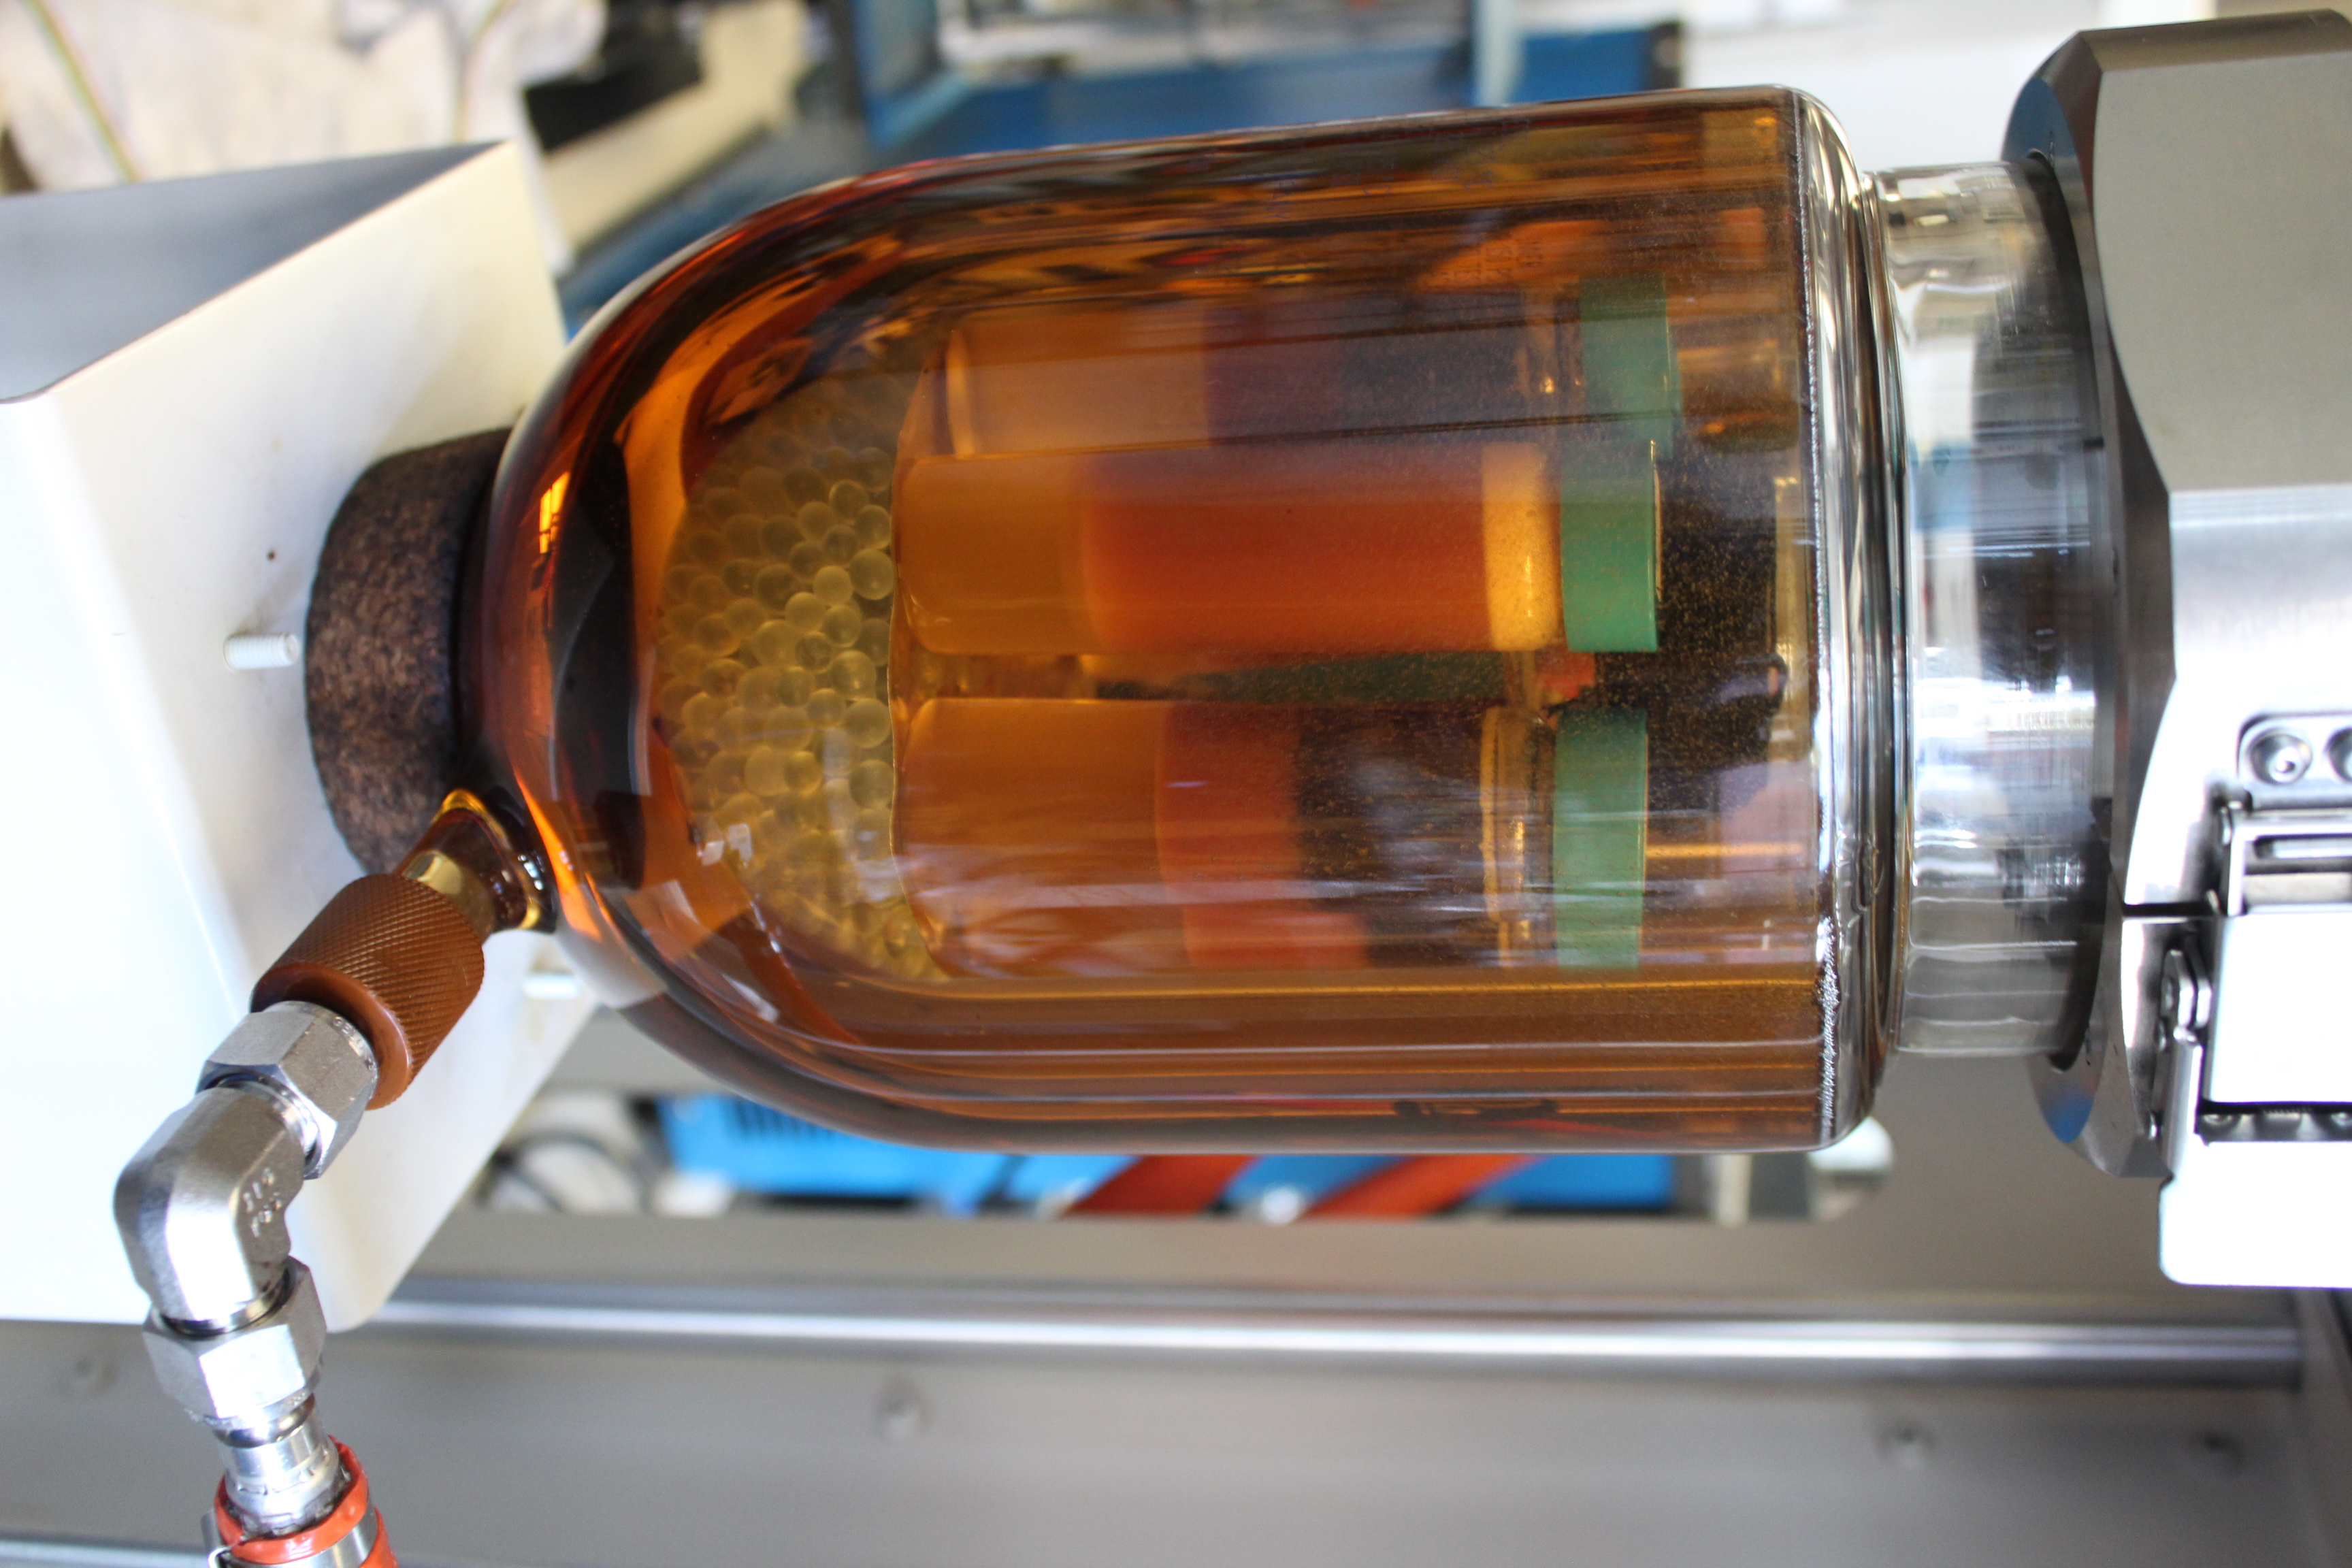
\includegraphics[width=0.5\textwidth]{Graphics/reactubos.JPG} } }
    \subfloat[]{
        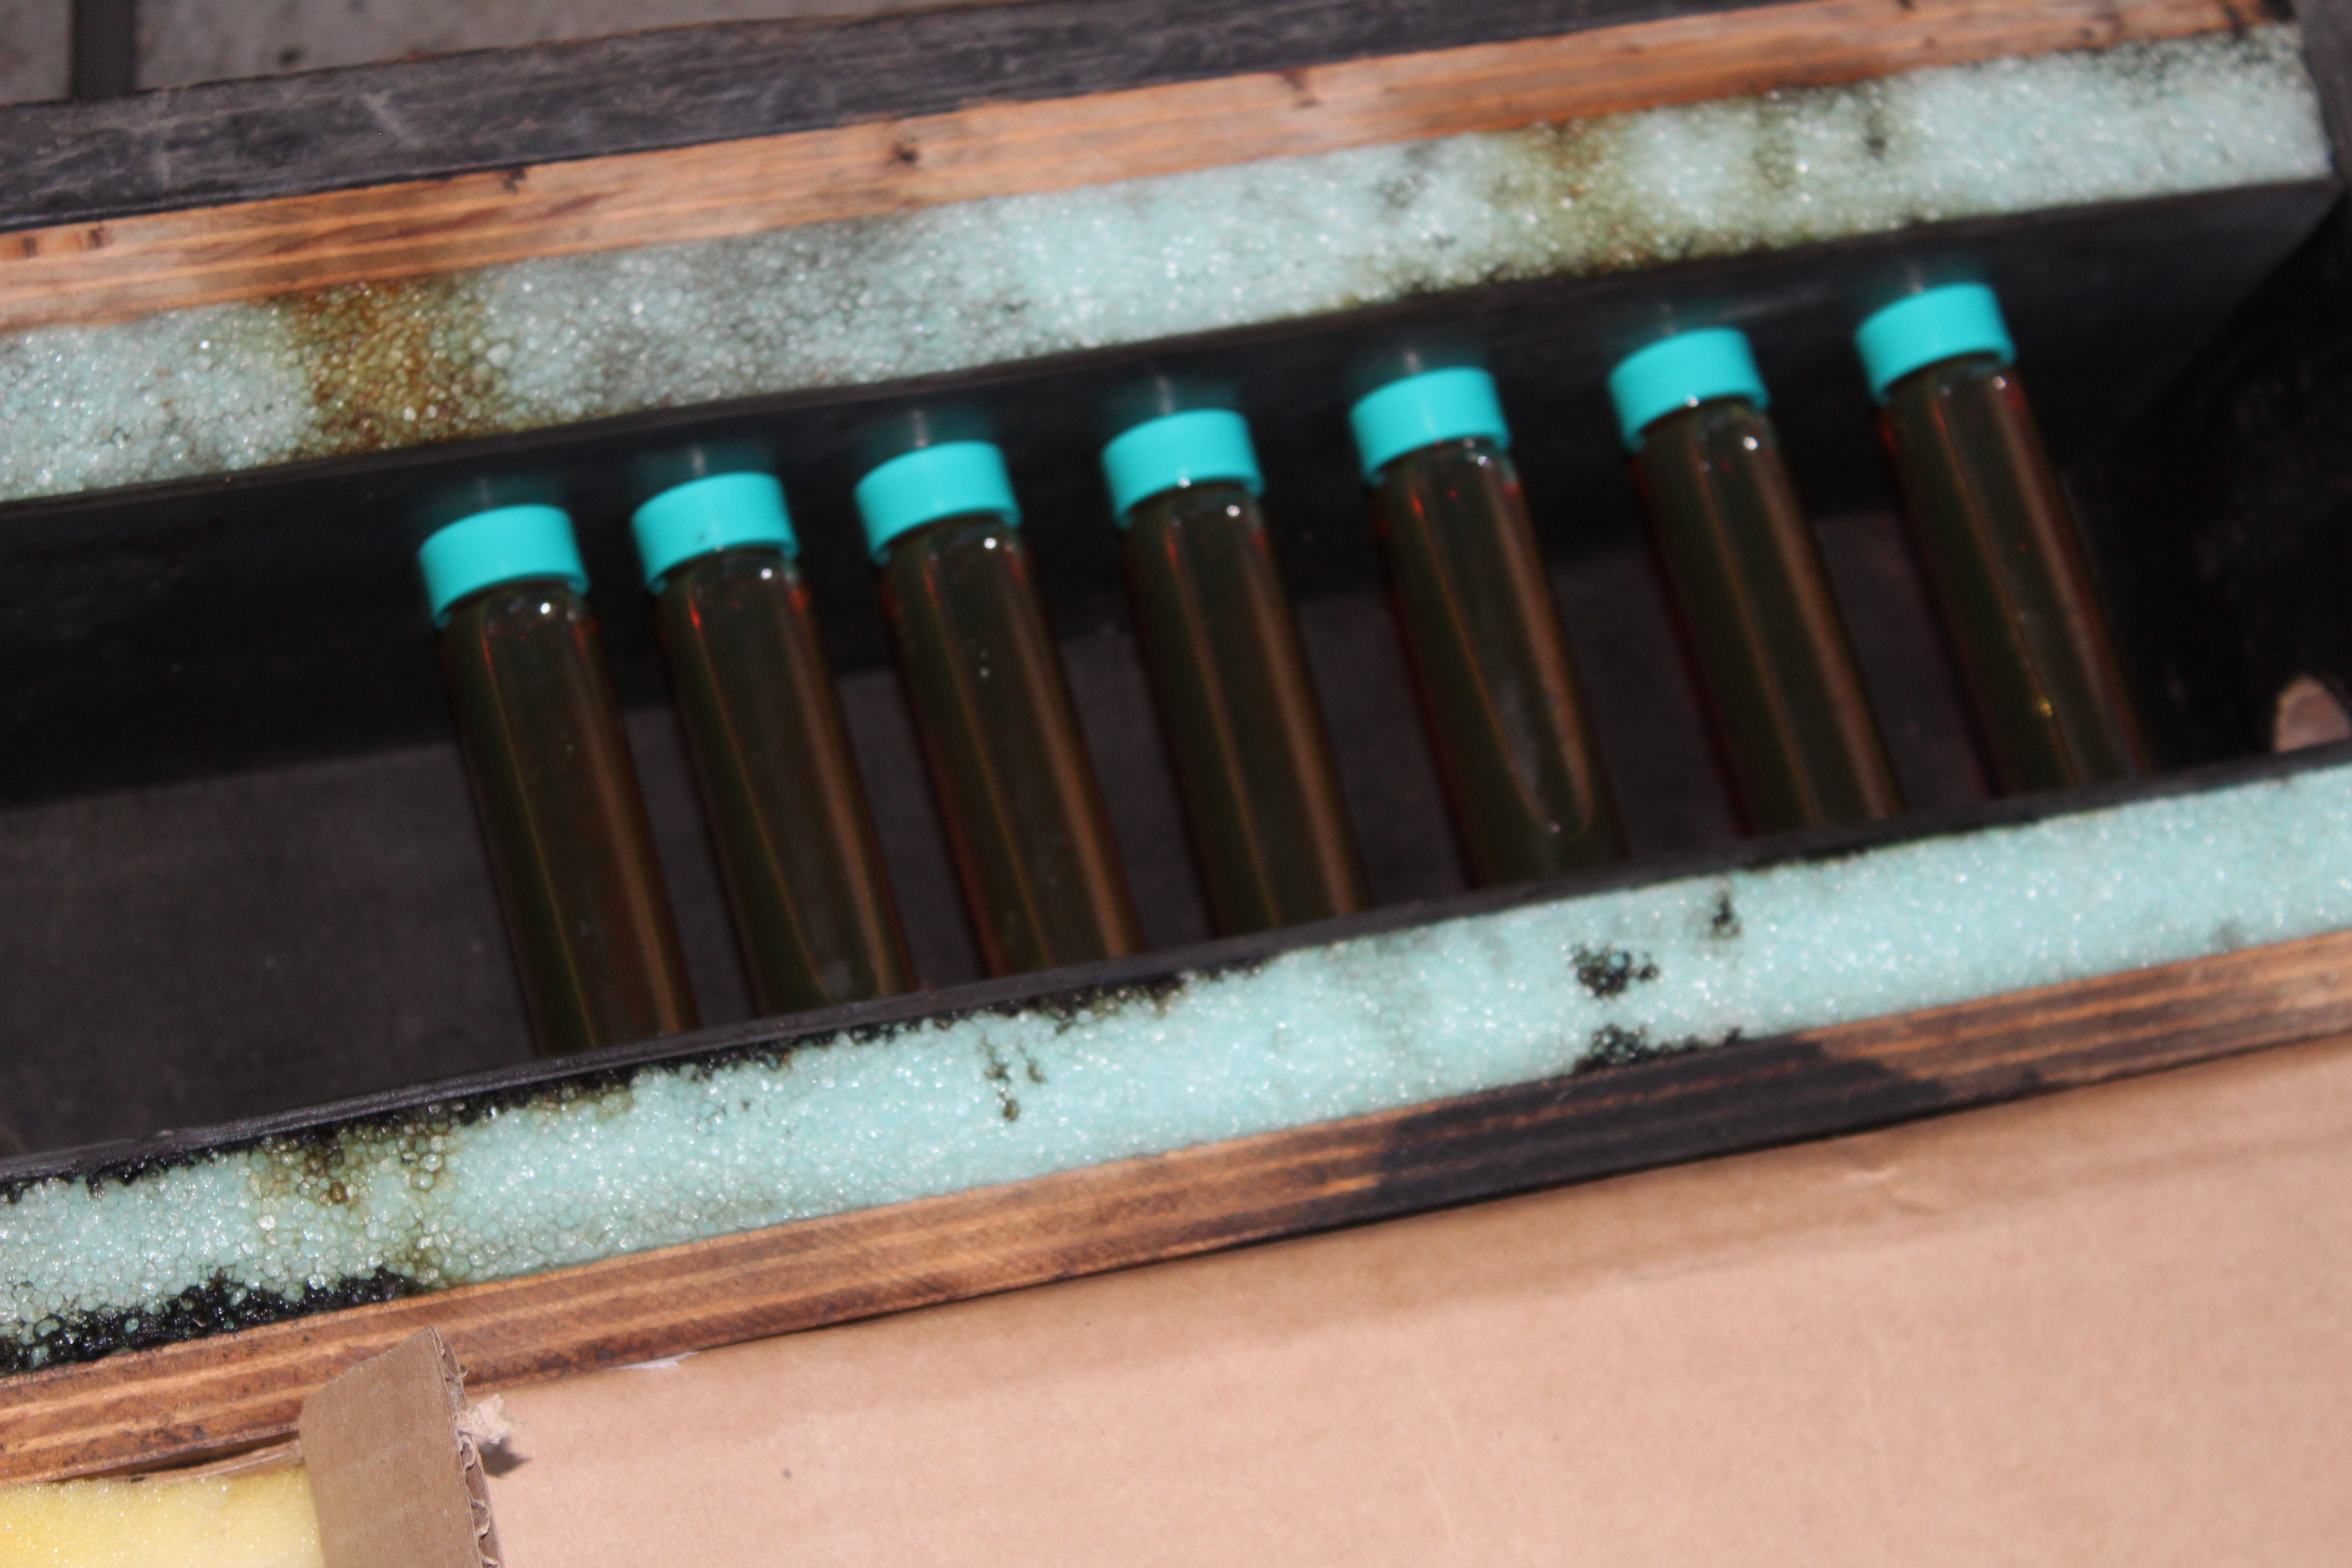
\includegraphics[width=0.5\textwidth]{Graphics/agitubos.JPG} }
    \caption[Muestras en tubos]{\textbf{(a)} Arreglo experimental en reactor Paar. \textbf{(b)} Agitador mecánico. }
    \label{fig:tubos}
\end{figure}

 \begin{table}[H]
    \caption[Pruebas de botella]{Serie $5$ Pruebas de botella del sistema A-S-S a diferentes concentraciones de surfactante.}
    \centering \footnotesize
    \begin{tabulary}{1.1\textwidth}{L |R|R|R|R|R|R|R}
        \toprule
        Botella & \textbf{1} & \textbf{2} & \textbf{3} & \textbf{4} & \textbf{5} & \textbf{6} & \textbf{7}  \\
        \midrule
        Concentración [\%] & $0.5$  & $1$ & $3$  & $5$ &$10$ & $13$ & $15$ \\
        Amesus ~~~~~~~~~~[ml] & $0.075$  & $0.15$ & $0.45$ & $0.75$ & $1.5$ & $1.95$ & $2.25$\\
        Salmuera ~~~~~~~~[ml] & $14.925$ & $14.85$ & $14.55$ & $14.25$ & $13.5$ & $13.05$ & $12.75$  \\
        Aceite ~~~~~~~~~~~~~[ml] & $15$ & $15$ & $15$ & $15$ & $15$ & $15$ & $15$  \\
        \midrule
        \bottomrule
    \end{tabulary}
    \label{tab:serie5}
\end{table}

Para cada serie se registra el nivel de las fases formadas en fotografías por $10$ días y mediante un algoritmo de conteo de pixeles, se registran los niveles de cada foto. Posteriormente se toma una muestra de cada fase formada y es montada en un microscopio.

\section{Tensión Interfacial}
Se llevaran a cabo mediciones de tensión interfacial en el sistema salmuera-aceite, aceite-aire, salmuera-organogel, y su comportamiento en con la concentración de surfactante. Esta información pretende ayudar a entender los procesos que ocurren dentro del sistema y permitirá complementar la descripción reológica. Para ello se utilizó un tensiómetro gota pendiente \emph{Krüss DSA} (\autoref{fig:Kruss}).
\begin{figure}\centering
    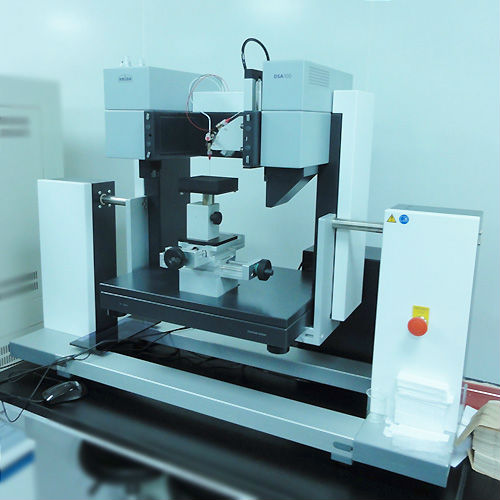
\includegraphics[width=0.6\textwidth]{Graphics/Kruss.jpg}
    \caption[Tensiómetro de gota]{Tensiómetro de gota pendiente Krüss DSA del Instituto Mexicano del Petróleo.}
    \label{fig:Kruss}
\end{figure}

Se prepararon $50$ ml de una solución madre de salmuera con $20000$ ppm de Amesus $3200$ en un matraz aforado, a partir de la cual se hicieron diluciones, el detalle de los volúmenes y concentraciones logradas se presenta en la \autoref{tab:diluciones}.

\begin{table}
    \caption[Diluciones]{Serie de diluciones a diferentes concentraciones de surfactante y salmuera.}
    \centering
    \begin{tabulary}{\textwidth}{|L|L|L|L|}
    \toprule
    Concentracion & \multicolumn{2}{c|}{Amesus 3200 } & Densidad \\
    \midrule
    ~ [ppm] & mg / $50$ ml & mg/ml & $\rho ~ [g/cm^{3}]$ \\
    \midrule
    20000 & 1000 & 20 & 1.15053 \\
    10000 & 500 & 10 & 1.15389 \\
    5000 & 250 & 5 & 1.15679 \\
    2500 & 125 & 2.5 & 1.15765\\
    1250 & 62.5 & 1.25 & 1.15936\\
    625 & 31.25 & 0.625 & 1.16064 \\
    325 & 16.25 & 0.325 & 1.16112 \\
    162.5 & 8.125 & 0.1625 & 1.16124 \\
    143 & 7.15 & 0.143 & 1.16133 \\
    65 & 3.25 & 0.065 & 1.161335 \\
    0 &0&0& 1.16140 \\
    \midrule
    \bottomrule
    \end{tabulary}
    \label{tab:diluciones}
\end{table}

Para la correcta determinación del diámetro de aguja utilizado, se utilizó un micrómetro con resolución de $0.01~mm$ y se calibro el sistema con agua tri-destilada y des-ionizada, de manera que a condiciones atmosféricas obtuviéramos el valor de tensión interfacial del agua, resultando en un diámetro de $0.9$ mm. En primer lugar se realizaron mediciones de tensión interfacial para el sistema Aire-Salmuera-Surfactante en todo el rango de concentraciones mostrado en la tabla anterior, utilizando como referencia el valor de densidad del aire al $16$ de mayo de $2017$ para la CDMX según el sistema meteorológico nacional que es de $1.1913264 kg/cm^{3}$.

Posteriormente se realizó la medición de tensión interfacial del sistema Aceite-Salmuera-Surfactante y finalmente para el sistema Salmuera-Organogel. Cada medición consiste de una fotografía de la gota, y su análisis mediante el algoritmo del equipo, similar al descrito en el \autoref{chp:antecedentes} de este trabajo.
